\section{Information System Overview}
\subsection{System components}
Figure \ref{System overview} gives an overview of the system components for sourcing, extracting, enriching and integrating the  data and making the resulting structured and higher level information available to the user's analysis.

\begin{figure}[h]
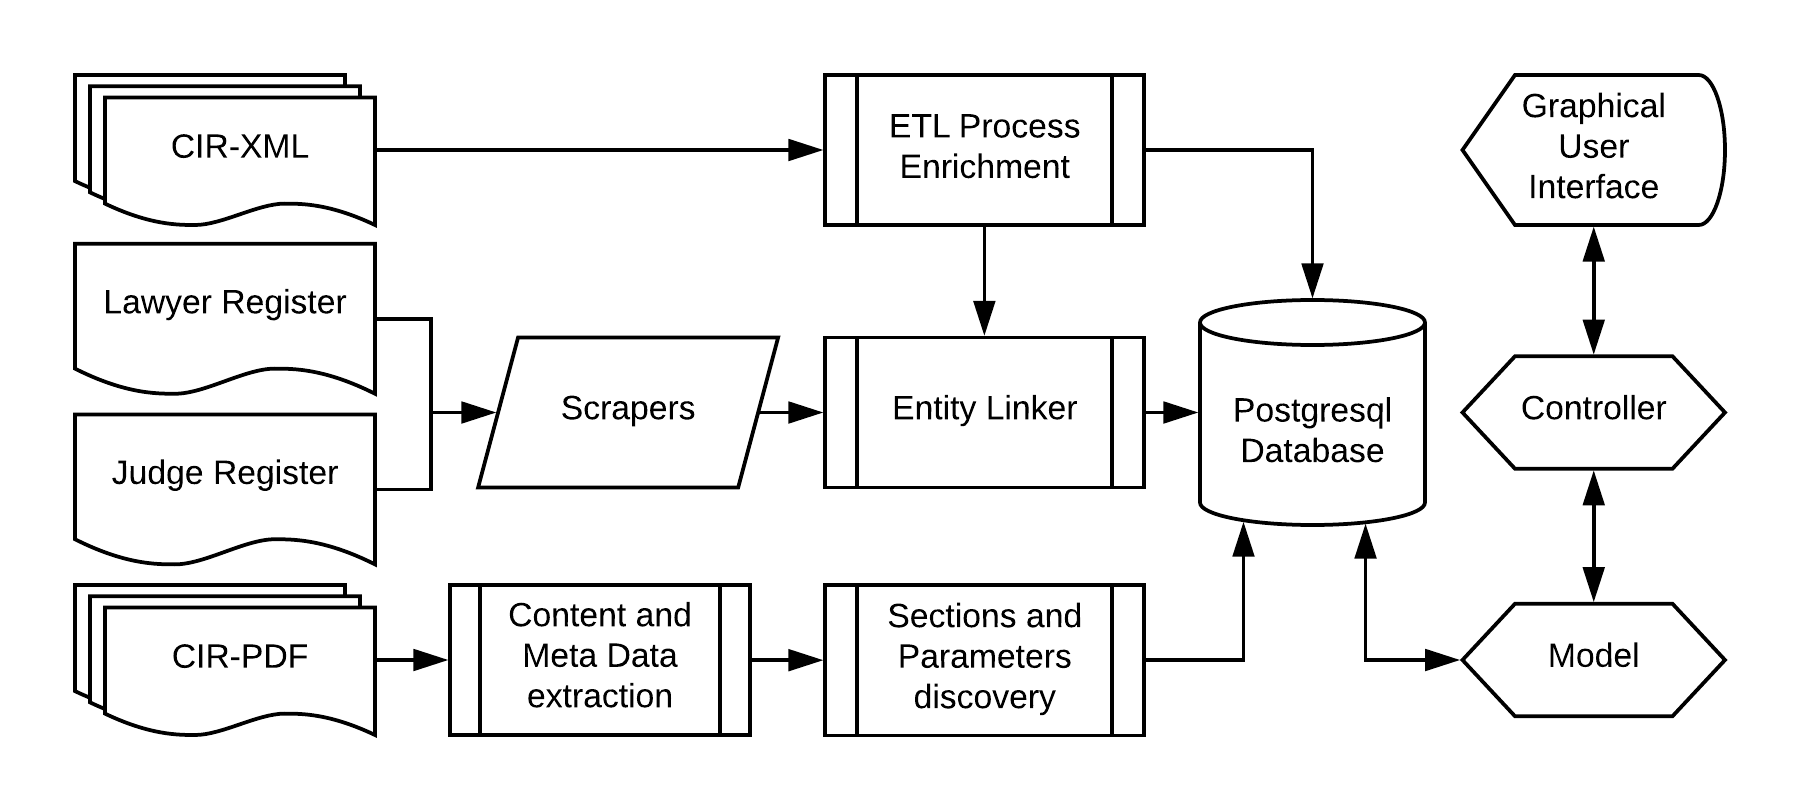
\includegraphics[width=1\linewidth]{images/system_overview.png}
\caption{System overview.}\label{System overview}
\end{figure}

Data flows from left to right through the following components:
\paragraph{Data Sources} Data is sourced from three public registers:
\begin{enumerate}
	\item The Central Insolvency Register (\textit{Centraal Insolventie Register or CIR}). CIR exposed both an XML and PDF file web service.
	\item The Register of lawyers (\textit{NOvA's Tableau}).
	\item The Register of ancillary positions of judges. (\textit{Register van nevenfuncties van rechters}) 
\end{enumerate}
The CIR provides the bulk of the data. The other two registers are used for the entity resolution of administrators and judges.

\paragraph{The ETL process and Enrichment} This component loads entities with selected data fields from the CIR XML data. The data is cleaned and enriched after which it is stored in a relational Postgresql database.

\paragraph{The Entity Linker} This component is responsible for linking judges and administrators in the CIR XML data to real life entities found in the judge and lawyer registers. 

\paragraph{PDF processors}
These component processes the CIR PDF reports to extract textual content and meta data. The text sections as defined in the progress report template and key data parameter are discovered in a subsequent process and loaded into the (Postgresql/Elastic) database.

\paragraph{Model-View-Controller (MVC)}
This well established pattern of subcomponents works together as a graphical interface for the user to analyse the data. 
%The user operates a graphical interface, prototyped in Jupyter notebooks, to query the data or interact with data visualisations or tables. The interface is the View in the MVC component. On user command, the Controller asks the Model to prepare the necessary data and then passes this data to the View to update the interface.

\subsection{Description of data sources}
\subsubsection{Central Insolvency Register}
\paragraph{Data suppliers}
The CIR \cite{rechtspraak:1} is operated by the state and contains company insolvency data supplied by the courts and the administrators. Courts are obliged to supply the insolvency data and free consultation thereof according to the insolvency law, article 19 \cite{law:1}. CIR started the register on the 1st of January 2005 and retains insolvency cases until six months after the ending of the insolvency.

\paragraph{Entities}
CIR data contain the following entities:

\begin{itemize}
	\item Courts
	\item Court Publications
	\item Supervisory Judges 
	\item Insolvency Cases
	\item Administrators
	\item Administrator Reports
\end{itemize}

\begin{figure}[h]
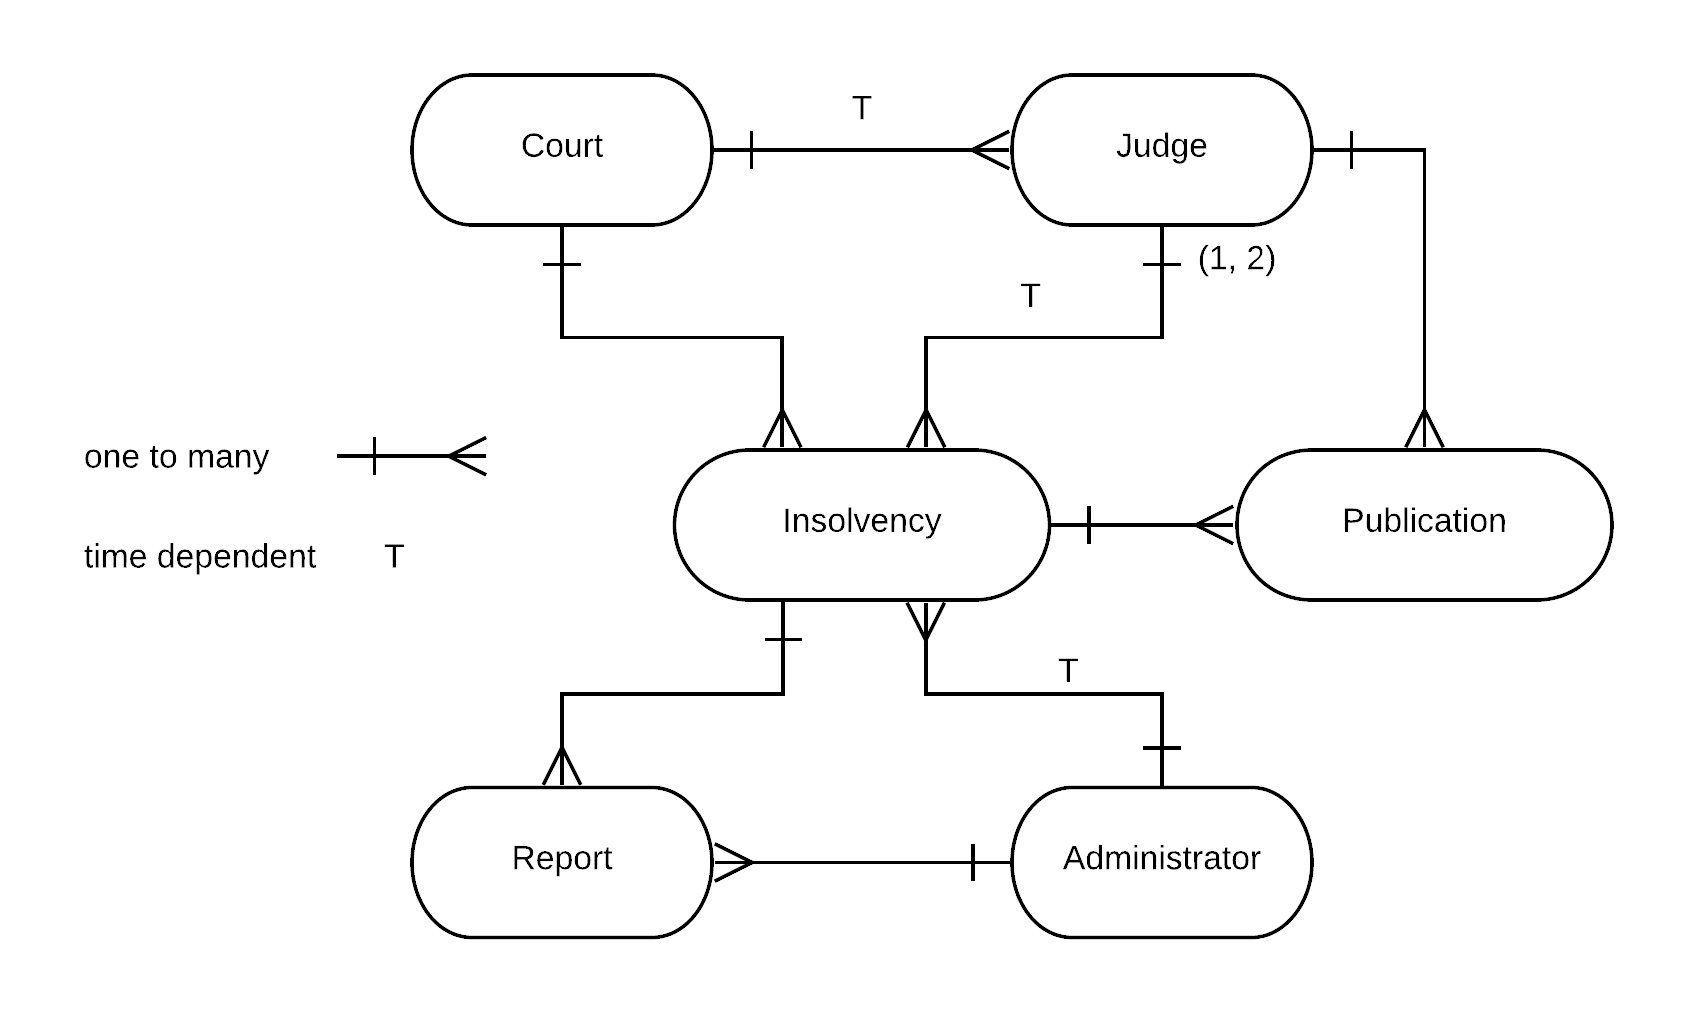
\includegraphics[width=1\linewidth]{images/cir_erd_2.png}
\caption{Insolvency entity relations.}
\end{figure}
\todo[inline]{remove law firm if not relevant. rename insolvent to insolvency}

\paragraph{CIR data contents}
Table \ref{table:cir_contents} shows the content of the CIR register data as of date [2018-08-12] and the average monthly size of new additions.

\begin{table}[h]
\caption{number of entity records and avg. monthly growth.}
\centering
\begin{tabular}{l r r}
\hline\hline
Entity & no. of records & delta\\
\hline
Insolvency & 17,331 & 280 \\
Report & 146,865 & 4408 \\
... progress report & 87,430 &  \\
... financial attachment. & 56,611 &  \\
Publication & 37,031 & 1447 \\
Administrator (distinct names) & 2329 & \\
Judge (distinct names) & 451 & \\
Court & 11 & \\
\hline
\end{tabular}
\label{table:cir_contents}
\end{table}
\todo[inline]{update numbers}

\paragraph{Identifiers}
The web service response in XML is semi structured data. It provides unique identifiers for Insolvency Cases, Publications and Reports	which can be stored in normalized SQL tables. The other entities Courts, Judges and Administrators have no identifiers but consist of free text fields for their name parts. These entities must be de-duplicated en linked to a real world entity.

\paragraph{Administrator Reports}
A second web service operated by CIR provides Administrator Reports in PDF format that hold much of the unstructured data. There are two types of reports: 
\begin{enumerate}
\item progress reports
\item financial attachments
\end{enumerate}
Recofa has published templates for both report types\cite{rechtspraak:3}.


\subsubsection{Register of lawyers, NOvA Tableau}\label{NOvA Tableau}
The NOvA tableau is the official register for lawyers and maintained by the \textit{Nederlandse Orde van Advocaten (NOvA)}\cite{nova:1}. Lawyers are obliged to be registered in the tableau by the lawyer's law (\textit{advocatenwet}, article 1 \cite{law:2}). NOvA offers an on-line search form where key word search and filters can be applied to search for a lawyer. This data source is used to collect the master data for Administrators. 

\subsubsection{Register of judges, Nevenfuncties van rechters}\label{Nevenfuncties Rechters}
The Register for ancillary positions for judges is made available by \textit{de Rechtspraak}\cite{rechtspraak:2}. It offers an on line form and returns the name, current and historical occupation and ancillary positions. This data source is used to collect the master data for Judges.